\chapter{Analyzing the Single Shot Detector}

Our goal is to improve SSD detector proposed by \citeauthor{bib:ssd} and adjust it to fit the needs of video surveillance.  We analyze the network and other performance impacting factors and try to find the improvements. We take an especially close look at the underlying convolutional network in SSD and compare multiple alternatives. The other important factor we consider is that the SSD was designed for detection on individual frames instead of a continuous video stream.

We base our work on the implementation of SSD by \citeauthor{bib:ssd}. However, since the performance of the neural network is heavily dependant on the used framework and hardware, and the precision depends on the training data, we had to re-implement and train the baseline SSD for our comparisons.

\section{Feature extraction network}
\label{sec:base}
Looking at the structure of the network, we found the best candidate for improvement to be the underlying feature extractor. The feature extractor provides the data on which SSD performs detection and is, therefore, the integral part of the model. SSD uses relatively old VGG-16 network that compared to more modern CNNs lacks in speed and precision.  The feature extractor is in the context of object detectors often called the \textit{base network}.

To explore the options, we started by implementing the SSD on multiple base networks and training them on the \textit{COCO} dataset to analyze the impact on SSD's performance. We decided to implement SSD on three 'post-VGG' networks, namely \textit{ResNet}, \textit{Xception} and \textit{NASNet}. 

We chose ResNet because it is a well-known network with simple design and easy scalability. Xception got our attention for its performance as a classification network in the benchmark by \citeauthor{bib:cnnbenchmark} (\cref{sec:cnncomp}), placing it around the optimal spot between speed and precision. NASNet, or precisely \textit{NASNet-A-Mobile}, was chosen out of curiosity for its unique, machine learning designed structure.

We will be referring to ResNet networks by their number of layers, e.g., ResNet50. Also, Xception will be called Xception version A, or shortly XceptionA, to avoid confusion with versions we are going to introduce later. To emphasize the base network of SSD network, we will be calling it \textit{base}-SSD, e.g., VGG16-SSD.

\subsection{Connecting SSD to other CNNs}
To implement the SSD on other base networks, we first needed to decide how to create the interface between the networks. We needed to define which features of SSD and the base network architectures we wanted to keep unchanged and which would have to be adjusted.

SSD uses six feature maps, two extracted from the VGG-16 network and four from extra layers. For input image of [300\x300] pixels, the feature map sizes are: [38\x38\x512], [19\x19\x1024], [10\x10\x512], [5\x5\x256], [3\x3\x256] and [1\x1\x256]. We decided to preserve the spatial resolution of feature maps as close as possible to the original, without changing the structure of base networks. Meaning, we did not keep the number of channels equal to SSD's. This approach certainly posed some risks. Not enough channels could negatively impact the precision, and too many channels would surely have an impact on the detection speed.

To find the most suitable layers for feature map extraction, we started with the strategy of finding the deepest possible layer with feature size as close as possible for every original feature map. This approach proved itself to be very straightforward since feature map sizes in convolutional networks decrease in resolution with the increasing depth, and the reduction is usually made by halving the size. After exhausting the network, we added the \textit{extra layers} as needed, similarly to VGG16-SSD. The final feature map sizes are listed in \cref{tab:features}. 

After determining the layers for feature extraction, we implemented the rest of the SSD without alteration. Each feature map fed into both classification and localization layer with the corresponding scale, as described in \cref{fig:VGGSSD}.

\begin{table}
    \centering
    \begin{tabular}{c|c|c|c|c}
        VGG-16 & ResNet34 & ResNet50/101 & XceptionA & NASNet* \\ 
        \hline
        38\x 512 &   38\x 128 &  38\x 512 &     37\x 256 &  28\x 264\\
        19\x 1024 &  19\x 256 &  19\x 1024 &    19\x 728 &  14\x 528\\
        10\x 512 &   10\x 512 &  10\x 2048 &    10\x 2048 & 7\x 1056\\
        5\x 256 &    5\x 512 &   5\x 512 &      5\x 512 &   4\x 512\\
        3\x 256 &    3\x 256 &   3\x 256 &      3\x 256 &   2\x 256\\
        1\x 256 &    1\x 256 &   1\x 256 &      1\x 256 &\\
    \end{tabular}
    \caption[Feature map sizes of SSD's base networks]{Feature map sizes used in SSD's detection. The dimensions are calculated for input image of [300\x300] pixels, with the exception of NASNet, which only accepts [224\x224] inputs. First number represents spacial dimensions of square feature and the second one represents the number of channels.}
    \label{tab:features}
\end{table}

\paragraph{ResNet} We had a bit of luck finding the right layers for feature extraction in ResNet networks. The high-level \textit{Layers} in ResNet produce features of [75\x75], [38\x38], [19\x19] and [10\x10] sizes. We simply picked the outputs of second, third and fourth layers and added appropriate feature layers after last \textit{Layer} for the rest of the features. The spatial dimensions of feature sizes are consistent on all ResNet version, with the only difference being the depth of the channels. The architecture of ResNet-SSD, with highlighted detection feature maps is illustrated on \cref{fig:resnet_xception_SSD}.

\paragraph{XceptionA} The high-level architecture of Xception, the entry, middle and exit flow, produce the features of [19\x19], [19\x19] and [10\x10] sizes. We can use the latter two outputs, but we had to step deeper into the entry flow and get the [38\x38] feature from the second block of the network. The network is topped by adding six extra layers that provide the remaining three feature maps. The XceptionA-SDD is illustrated on \cref{fig:resnet_xception_SSD}.


\begin{figure}
    \centering
    \resnetSSD
    \caption[Resnet34-SSD and Xception-SSD]%
    {Resnet34-SSD(left) and XceptionA-SSD (right). For details on \textit{Layers} and \textit{Blocks} see \cref{fig:resnet_arch} and \cref{fig:xception} respectively. Extra layers are highlighted with a red dashed rectangle.}

    \label{fig:resnet_xception_SSD}
\end{figure}

\paragraph{NASNet} The architecture of NASNet has proven to be the trickiest one for implementing SSD. Even though it is a fully convolutional network, due to the complex structure with many additions and concatenations, it does not accept any input except for [224\x224] pixels. Rather than doing large scale changes to the architecture, we decided to compromise on the detector side and use the lower resolution. 

Other than the input size, the next problem of the NASNet-A-Mobile is the lack of choice of feature maps for detection. Because the stacks of Normal Cells do not change the spatial dimensions, there are only three available sizes of feature maps. Without any real choice, we end up with features of [28\x28], [14\x14] and [7\x7] sizes. The problem here is that [7\x7] feature map has only enough pixels for two subsequent [3\x3] convolutions. Therefore we had to implement SSD with only five feature layers for detections. See \cref{fig:nasnetSSD} for architecture details.


\begin{figure}
    \centering
    \nasnetSSD
    \caption[NASNet-SSD]%
    {NASNet-SSD based on NASNet-A-Mobile. The network is limited to input of size [224\x224] due to complex structure of NASNet cells. For detailed description of cells see \cref{sec:nasnet}.}
    \label{fig:nasnetSSD}
\end{figure}

\subsection{Performance results}
We trained the SSDs on COCO dataset, to compare their performance, both in terms of precision and speed. The base networks we choose to compare are VGG-16, ResNet34, ResNet50, ResNet101, XceptionA, and NASNet-A-Mobile. For a relevant comparison, all networks were implemented in the same framework and trained for an equal number of iterations. We can see, from the results in \cref{fig:cocoperf}, that VGG-16 is outperformed by all of our choices in terms of speed, but overcomes the XceptionA and NASNet in precision. 

We believe that the compromises we had to make in implementing NASNet-SSD, the smaller input image resolution, fewer feature maps for detections, are the reason for the poor precision performance. Concerning XceptionA, we hypothesize that we extract the first feature map from a too shallow layer, after passing only six convolutional layers. If the first feature map is compromised, that would impact the detection of small objects and have a substantial impact on the precision. We will test our hypothesis and try to rectify the problem of Xception-SSD in \cref{sec:fixxception}.

\begin{figure}
    \centering
    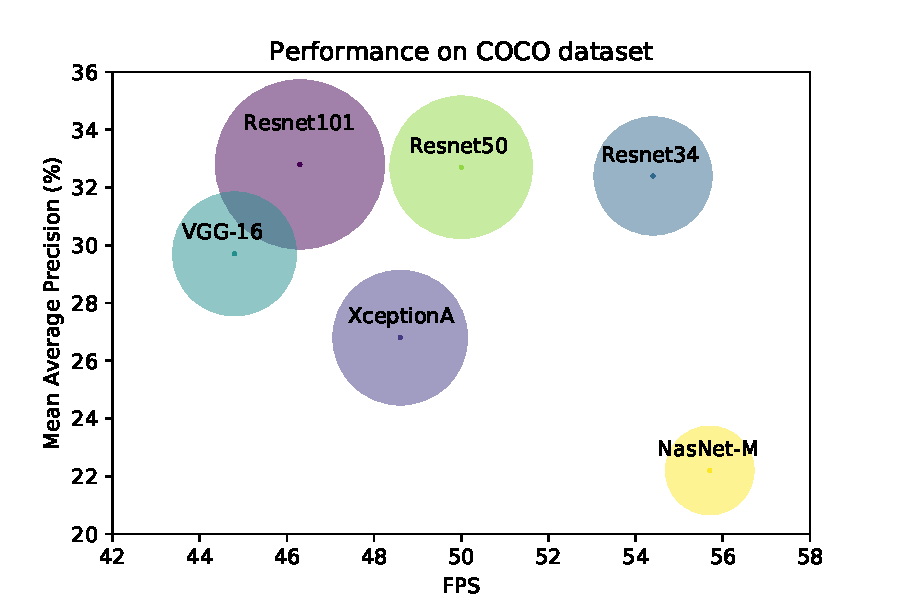
\includegraphics[width=\textwidth]{img/fps_map_c}
    \caption[Performance of SSD with multiple base networks on COCO dataset]{Performance of SSD detector on multiple base networks. Circle diameters demonstrate relative difference of network parameter counts.}
    \label{fig:cocoperf}
\end{figure}

\section{Training data and classes}
The main problem of solving problems with neural networks is the lack of available data. Some problems can be solved by reinforcement learning, but others, like object detection, need supervision. The creation of a custom problem-specific dataset requires a lot of human resources and is viable only for big companies. Therefore, dependent on public datasets like COCO. The problem of such datasets is that they often include many classes that are not needed for a particular application. For surveillance, we are interested in classes such as people and vehicles. We are going to compare the performance and precision of SSDs between training on full COCO dataset and a subset for surveillance. We expect significant performance improvement by lowering the number of detector classes. However, we were not sure how will this change impact precision. 

\subsubsection{Surveillance dataset classes}
\begin{multicols}{2}
    \begin{itemize}
        \item person
        \item bicycle
        \item motorcycle
        \item car
        \item bus
        \item truck
        \item train
    \end{itemize}
\end{multicols}

\subsection{Precision impact}
Training a network on a subset of larger dataset seems to be a straightforward task. However, we hypothesize that by removing classes with similar features to the ones we are detecting, there is a possibility of increasing the error on those selected classes. 

For example, consider a dataset of humans and monkeys. The networks learn to distinguish between the two and classify everything else as a background. If we do not care about monkeys, we can filter them out in post-processing. However, consider a network that is trained only to recognize people and use it on a monkey. We are worried that such a network would classify a monkey as a person, based on a large number of similar features. 

To counter-measure the possibility of a larger amount of false positives, we decided to increase the number of negative samples. We did it by only filtering annotation from \textit{COCO} dataset to create the \textit{surveillance dataset}, but keeping all the images, even those without positive ground-truths. The expectation is to reach similar precision on selected classes, on both \textit{COCO} and \textit{surveillance dataset}. However, because \textit{COCO} is a small dataset with only about a hundred thousand images and is certainly not exhaustive in classes with similar features to \textit{surveillance dataset}, this measure would only help on our evaluation data.

\paragraph{Results} in \cref{tab:ssdcocosurv} show that it is possible to remove unnecessary classes from the dataset without impacting the performance. We tested the approach on multiple architectures, and the results do not conclusively favor one dataset over the other. 

\begin{table}[]
    \centering
    \begin{tabular}{c|c|c}
         & COCO & Surveillance  \\
         \hline
        ResNet34 & 47.3 & 47.3 \\
        ResNet50 & 46.6 & 48.7 \\
        ResNet101 & 47.2 & 45.7 \\
        XceptionA & 39.4 & 37.8 \\
        NASNet & 36.4 & 36.9 
    \end{tabular}
    \caption[SSD's precision comparison between COCO and surveillance datasets]{Mean average precision of \textit{surveillance} classes. Comparing networks trained on all 80 classes of \textit{COCO} dataset and \textit{surveillance} subset of \textit{COCO}.}
    \label{tab:ssdcocosurv}
\end{table}

\subsection{Performance impact}
We expect a proportional increase in performance with the removal of the classes. We saw that in the SSD (\cref{fig:VGGSSD}) the depth of the classification layers is dependent on the number of classes. Another important factor is that smaller dimensions of detection tensors will result in faster post-processing, i.e., non-maximum suppression. 

We illustrate the effect of the number of detected classes on performance on \cref{fig:fpscls}, based on measured data. Although the relationship of frames per second and classes is hyperbolic, on the interval between 7 and 80 classes, we approximate the loss of 0.78 frames per second per class on ResNet50-SSD. This is a significant number and means that training the networks for particular purposes can bring a substantial benefit as opposed to using a general detector for everything.

\begin{figure}
    \centering
    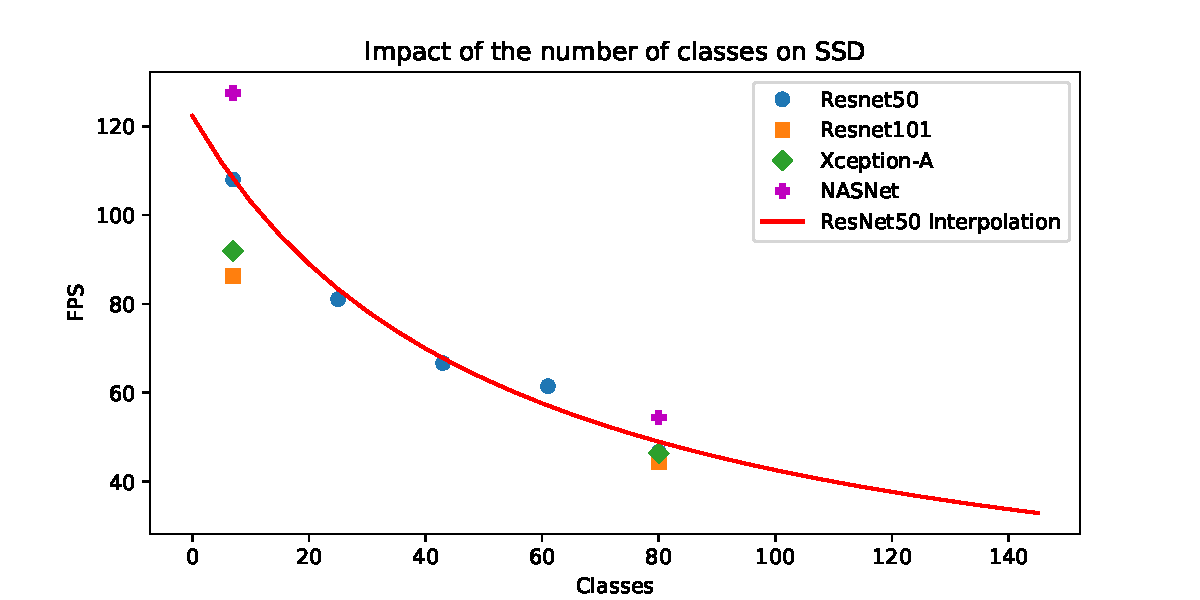
\includegraphics[width=\textwidth]{img/fps_cls}
    \caption[Impact of the number of classes on SSD performance]{Impact of the number of classes on SSD performance. Inference time values ($1/fps$) are linearly interpolated, the result is therefore hyperbolic approximation of frames per second.}
    \label{fig:fpscls}
\end{figure}


\section{Modifying Xception}
\label{sec:fixxception}
We managed to successfully re-implement SSD on other architectures and boost the speed of surveillance by removing unnecessary classes. We can confidently say that ResNet50-SSD with 48.7\% mAP and 108fps or ResNet34-SSD with 47.3\% mAP and 125fps outperform original SSD on VGG-16 with 46.1\% mAP and 42fps. However, we believed that the underwhelming result of XceptionA-SSD could be used as a stepping stone and the results could be pushed further with modifications to the base network architecture. We did not try to improve upon NASNet-SSD because of limitations described in \cref{sec:base}.

We believe that the major factor limiting the precision of XceptionA-SSD is the extraction of [37\x37] feature map after the second block of the network. To rectify this problem, we decided to make adjustments to the network, so that we could extract [37\x37] feature map after \textit{block 7}, and keep the [19\x19] map after \textit{block 11} as previously dictated by network architecture. The reasoning behind choosing \textit{block 7} was that it is deep enough in the network and leaves four blocks between the feature map extractions. It is perhaps a bit arbitrary decision and blocks 6 or 8 would do just as well, or better.  In order to achieve the correct sizes of feature maps, we moved the max-pooling with stride 2 from \textit{block 3} to \textit{block 8}. This resulted in outputs of the \textit{block 2-7} to be the 37\x37 size and \textit{block 8} to output 19\x19 feature map. 

The proposed change to the pooling, and thus feature map sizes results in the increased complexity of the network as the [19\x19] features with 728 channels now grew to the [37\x37] size. To remedy this, we decreased the number of channels for concerned blocks to 256. We also decided to continue with trimming layers in the rest of the network. In the end, we got the [37\x37] map with 256 channels, [19\x19] map with 512 channels and [10\x10] map with 1024 channels. The architecture with highlighted changes is illustrated on \cref{fig:xceptionH_SSD}. 

Our modification not only helped to improve Xception-SSD to overcome VGG-16, but we also outperformed ResNet50-SSD's 48.7\% mean average precision with 49.8 \% mAP. However, despite our best efforts to save computation, we managed to outperform XceptionA only slightly by achieving 92fps. The relative performance of XceptionH based SSD to other SSDs using the \textit{surveillance dataset} can be seen on \cref{fig:surv_perf}.

\begin{figure}
    \centering
    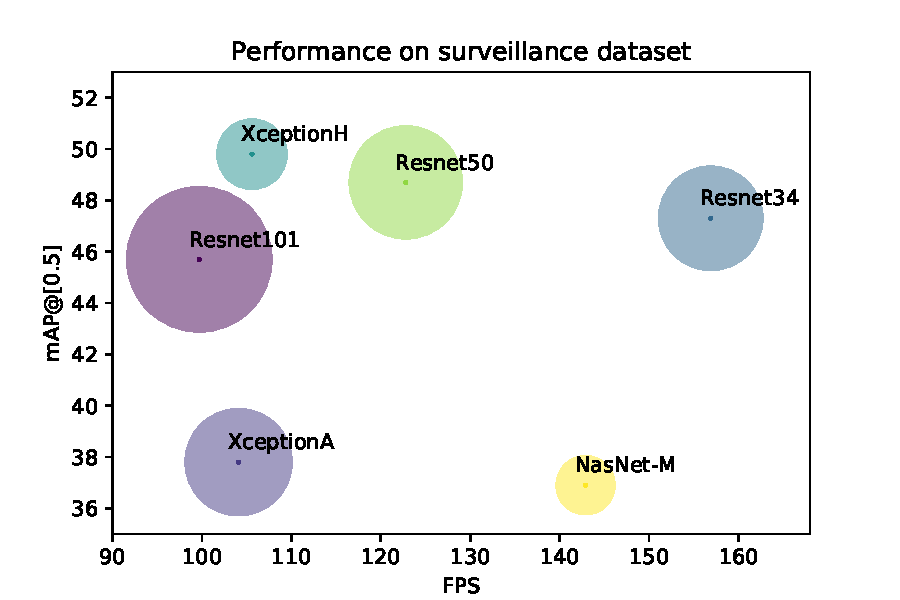
\includegraphics[width=\textwidth]{img/fps_map_s}
    \caption[Performance of SSD with multiple base networks on Surveillance dataset]{Performance of SSD detector on multiple base networks. Circle diameters demonstrate relative difference of network parameter counts.} 
    \label{fig:surv_perf}
\end{figure}

\begin{figure}
    \centering
    \xceptionSSD
    \caption[XceptionH-SSD]%
    {XceptionH architecture (right) compared to XceptionA (left). Changes are highlighted with bold font. Connection to SSD's detection layers are indicated by the arrows on the sides, extra layers are appended to the bottom of the network.  \textbf{S} represents stride of the block, implemented using max-pooling. Blocks are also color-coded based on the feature map size. Extra, classification and localization layers are unchanged from \cref{fig:resnet_xception_SSD}. For details on \textit{Blocks} see \cref{fig:xception}.} 
    \label{fig:xceptionH_SSD}
\end{figure}




\section{SSD-TC: SSD with temporal convolution}
Our main priority is video surveillance, which means the detection in video. We already explored two approaches to exploiting the continuity of video frames to achieve higher precision in \cref{sec:video_det}. One approach used network similar to \textit{Faster R-CNN} with use of temporal tubes-of-interest. The other one used \textit{Single Shot Detector} and modified it with convolutional LSTM cells to harness the temporal information. However, the major drawback of both approaches was their inference speed. 

Inspired by the two approaches, we decided to implement our video detector with temporal information. To this end, we chose to expand on the SSD as we already have the understanding of the model and the single-stage models are currently the only relevant choice considering speed. We also wanted to avoid adding complex, time-consuming structures like LSTM cells used in TSSD. Instead, decided to use three-dimensional convolutional layers, to aggregate the information from multiple images. We named our approach \textit{Single Shot Detector with Temporal Convolution} (SSDTC).

Of course, we need to prove our concept by training it on some data and comparing it to unmodified SSD. Because we need a dataset with consecutive frames, we decided to start with the \textit{HollywoodHeads} dataset. This set annotates heads in sections of movies. Considering that dataset has only one class and previous results of SSD testing, we trained ResNet34-SSD as a baseline. Therefore, we also based SSDTC on ResNet34-SSD.

\subsubsection{Architecture}
Unlike batching of independent images, we expect to perform detection on a single batch, or a chunk, of consecutive frames. We extract the feature maps, as we would in SSD, independently on each frame with the same network. Starting with the chunk \textit{n} = 16, we get 16 sets of feature maps. Considering only the first feature map of [38\x38\x c] size, stacking those maps from the whole chunk we get a temporal feature volume of [38\x38\x n\x c] size, where \textit{c} is the number of channels. At this point, we apply the temporal convolutional layers, realized using 3d convolutional layers (conv3d). We apply two conv3d layers. First one works only with temporal and channels dimensions, with filter shape [1\x1\x3\x ch].  The other one works with all dimensions of feature volume, with [3\x3\x3\x2*ch] shape. Both layers are followed by batch normalization and ReLU activation. No padding is used in the temporal dimension of conv3d layers, therefore we only receive \textit{n-4} detections for \textit{n} input frames. This may seem inefficient because five frames are needed for detection on one frame, but the impact of this constant overhead can be minimized with bigger chunks. After the temporal layers, we can again view the created feature volume as an array of independent frames and apply SSD's detection layers. 

In simple terms, we add temporal information from neighboring frames to each feature map, before executing the detection. This allows for reuse of most of the SSD's architecture and simple transition on other base networks. The illustration of SSDTC's architecture can be seen on \cref{fig:ssdtc}.

\begin{figure}
    \centering
    \ssdtc
    \caption[Single Shot Detector with Temporal Convolution]{SSDTC architecture on ResNet34 base. All temporal layers are followed by batch normalization and ReLU activation functions.}
    \label{fig:ssdtc}
\end{figure}


\subsubsection{Results}
A previously mentioned, ResNet34-SSD was trained on the same dataset to serve as s baseline for comparison. This SSD achieved the precision of 81.6\% while performing at 156 frames per second. 

Our SSDTC architecture managed to reach the precision of 86.9\% with processing speed of 148 fps. However, considering that detection is not performed for every processed frame, the effective speed of the network is 111 frames per second with the chunk size of 16 frames. 
